\chapter{Results and Discussion}

\section{Cultivation of Bacteria\authorB}
Upon acquisition of the bacterial strain, it underwent cultivation on agar plates followed by
incubation. However, initial observations within the first week of incubation did not yield
satisfactory results, as Methylorubrum Extorquens (M. Extorquens) failed to produce a visibly
discernible orange culture indicative of successful growth.

By the third week of cultivation, a distinct orange dot appeared on the surface of the incubated
agar plate, signifying the emergence of bacterial growth. The bacteria were meticulously scraped
from the solid nutrient media for subsequent cultivation in liquid nutrient media, thereby
facilitating a transition from solid to liquid growth conditions.

\begin{figure}[H]
    \centering
    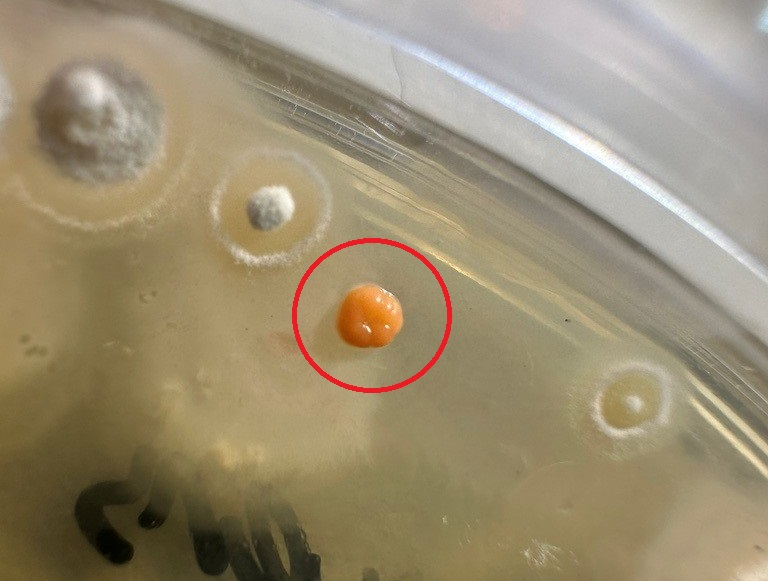
\includegraphics[width=0.9\textwidth]{./media/images/first_mextorquens}
    \caption{First \emph{M. extorquens} culture developed from an acquired strain.}
    \label{fig:first_mextorquens}
\end{figure}

Subsequent growth in liquid media exhibited a remarkable proliferation of bacterial colonies. To
maintain optimal growth conditions and prevent overpopulation-induced stress, a routine
procedure of decanting 75\% of the liquid culture from the flasks and replenishing them with fresh
liquid media was implemented on a weekly basis. This critical step ensured the sustained viability
and productivity of the bacterial population.

Toward the latter stages of the project, flasks were emptied completely, yet bacterial colonies
regenerated solely from residual deposits adhering to the inner walls of the flasks.

It was also observed that the addition of Methanol had a significant impact on \emph{M. extorquens}’
growth speeding up it’s growth by 20\%-50\%, this is explainable by \emph{M. extorquens}’ methanol
metabolizing capabilities.

\section{Protein Analysis\authorA}

With the analysis of the lysed bacteria, we wished to be able to determine if the bacteria are capable of producing LanM.
We tried two methods for protein analysis, namely the IR-Spectrometry and the SDS-PAGE.
However, both methods did not bring any valuable results.

\textbf{IR-Spectrometry}

The IR spectra of our samples looked all the same, and they did not have any significant differences.
In general, all spectra showed the lysis buffer we used to lyse the bacteria (see figures~\ref{fig:ir_spectrum_2} and~\ref{fig:ir_spectrum_1}).

\begin{figure}[H]
    \centering
    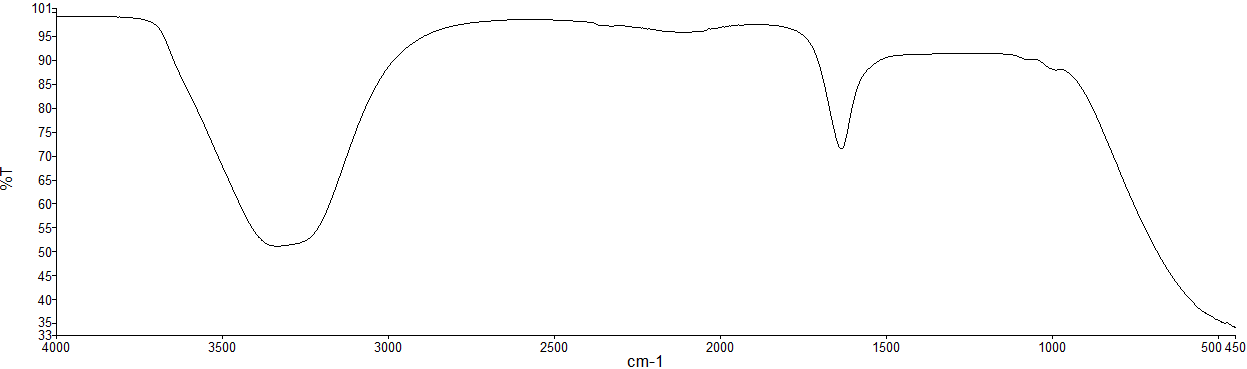
\includegraphics[width=1\textwidth]{./media/images/ir_spectrum_2}
    \caption{IR-Spectrum of proteins solved in water, from a culture of \emph{M. extorquens}, to which no rare earths were given. }
    \label{fig:ir_spectrum_2}
\end{figure}

\begin{figure}[H]
    \centering
    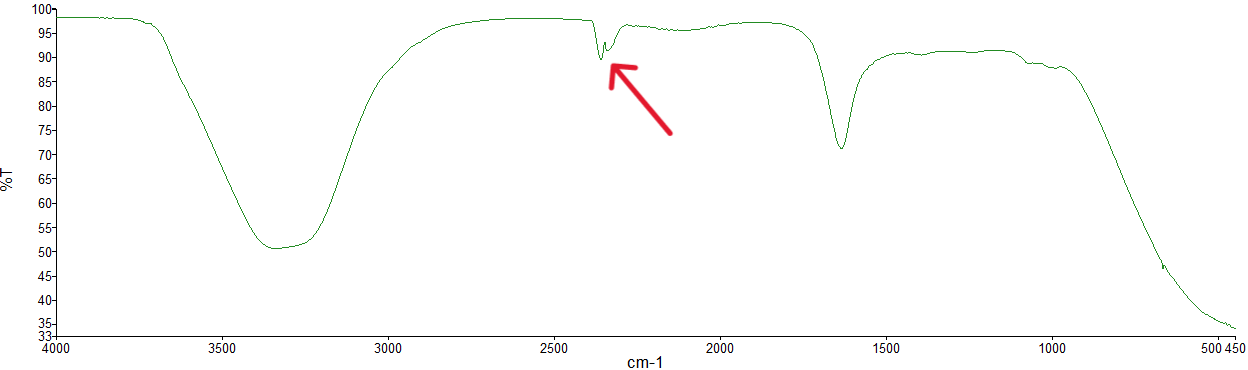
\includegraphics[width=1\textwidth]{./media/images/ir_spectrum_1}
    \caption{IR-Spectrum of proteins solved in water, from a culture of \emph{M. extorquens}, to which the \ce{NdFeB}-solution was given. The marked valley stems from the wrongly calibrated IR-Spectrometer. }
    \label{fig:ir_spectrum_1}
\end{figure}

There were no results because maybe we did not have enough amounts of bacteria, which would have more proteins, to make their spectra more visible.
It could also be that we did not achieve to break the cell wall of enough bacteria, so that we could analyze the proteins.

\textbf{SDS-PAGE}

The SDS-PAGE was really challenging to perform, because most of the time, the gel did not polymerize.
This could be due to old chemicals, or the chemicals did not have the right temperature to link and form the gel.
However, we tried the SDS-PAGE multiple times, and we did not find the correct reason why our gel sometimes polymerized and sometimes not.

\begin{figure}[H]
    \centering
    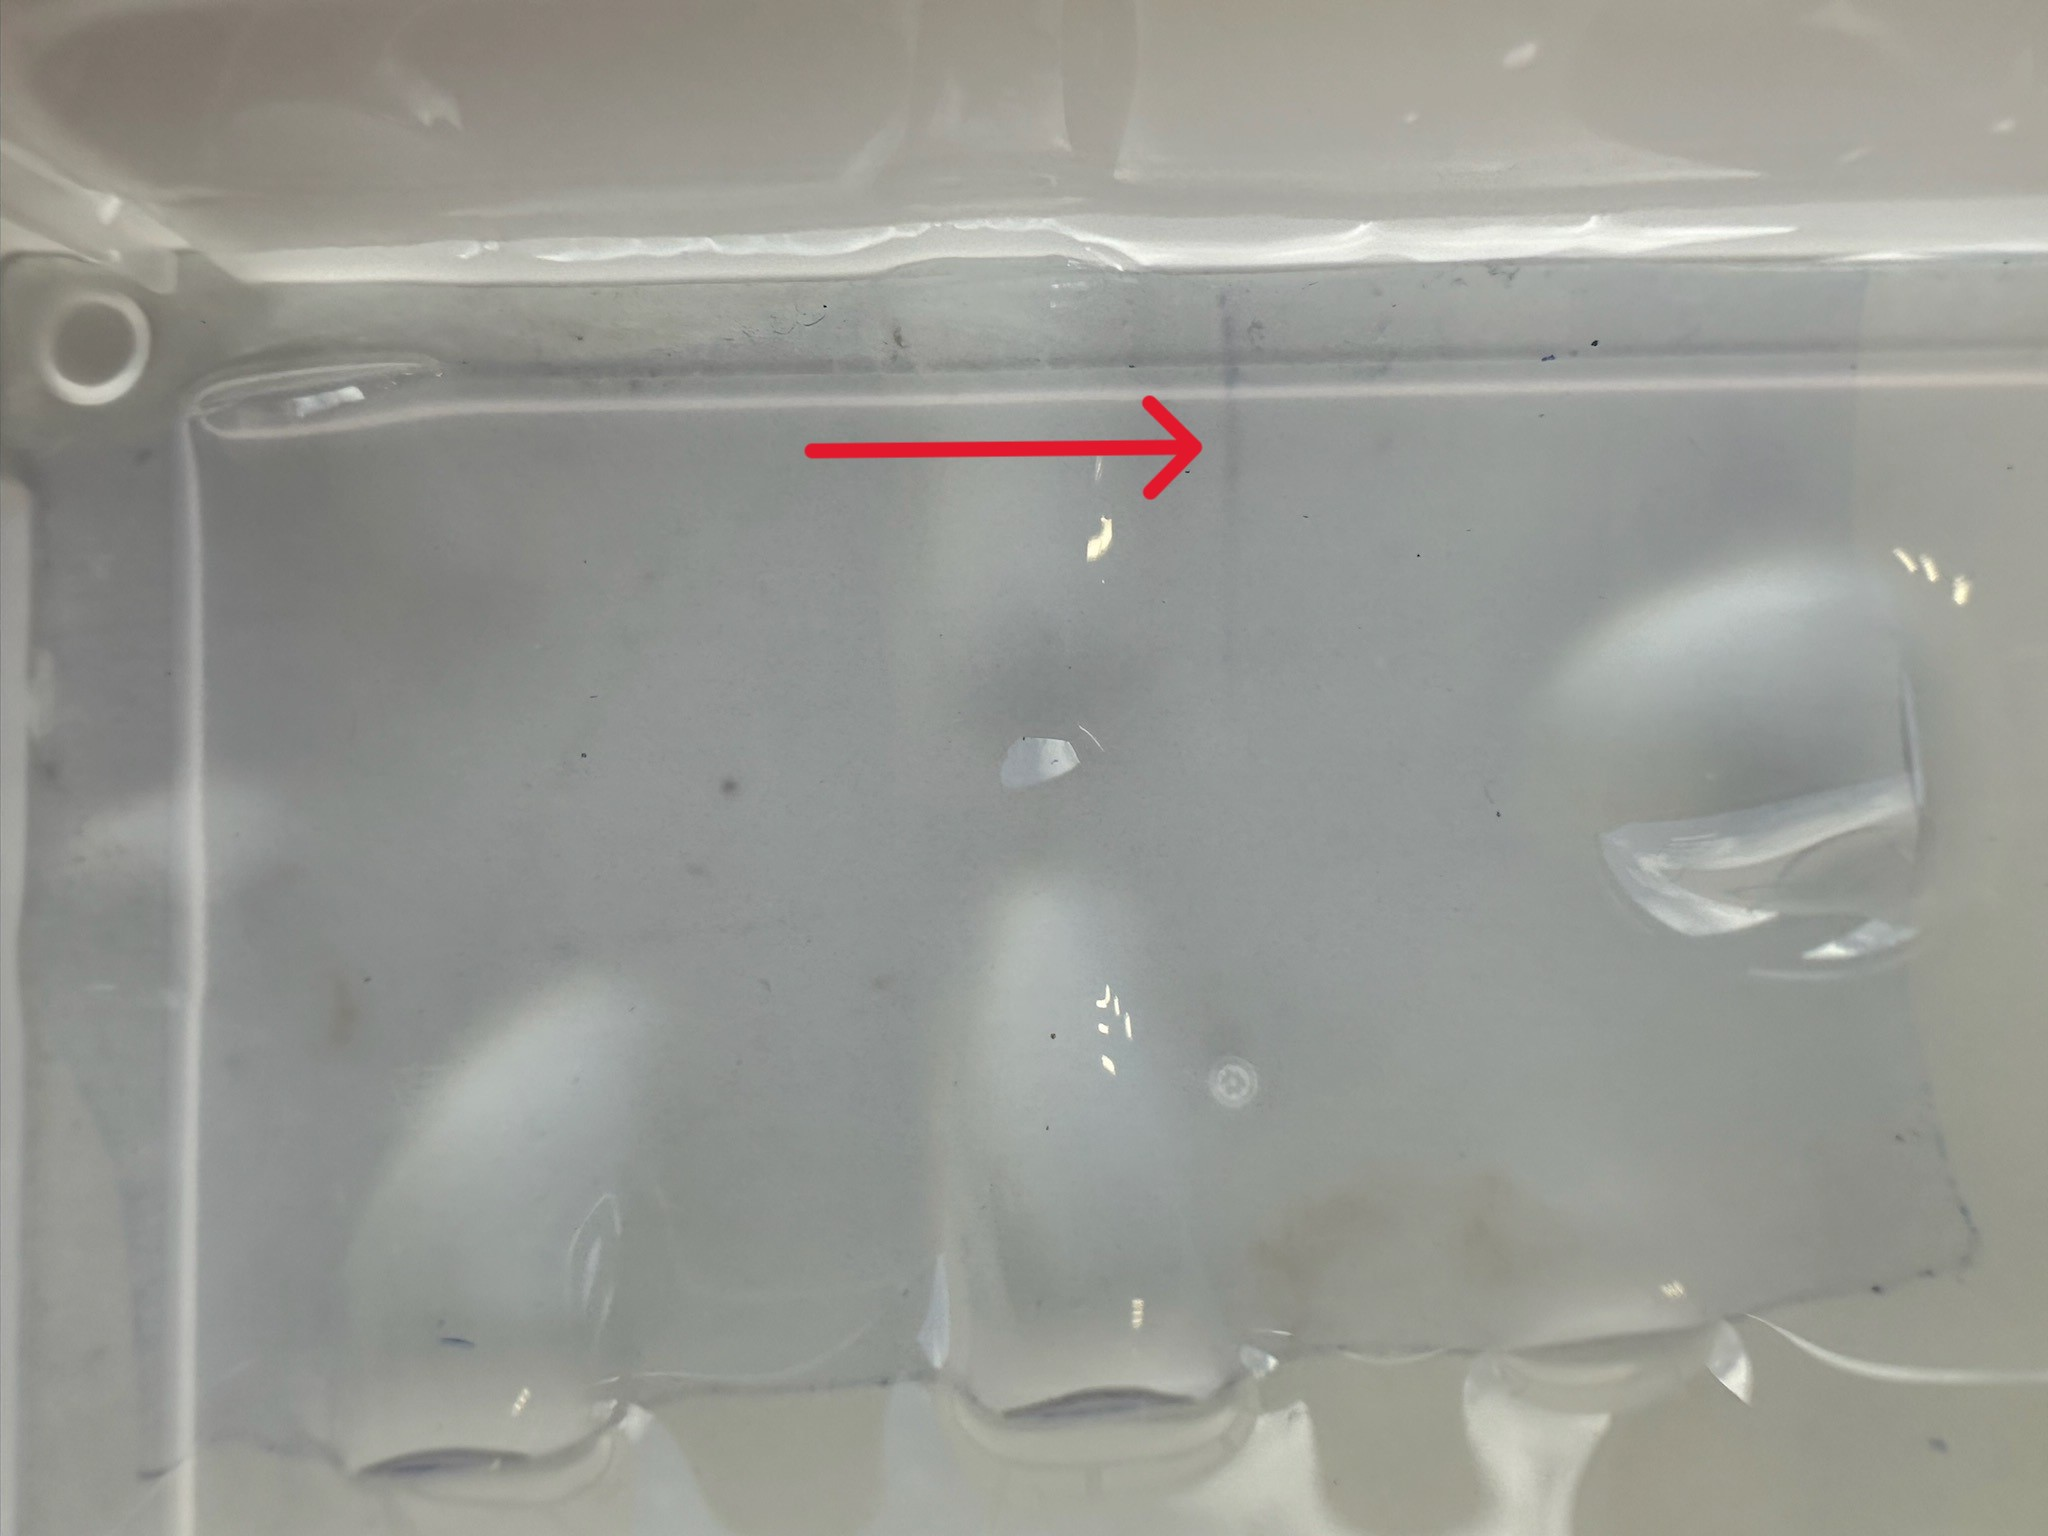
\includegraphics[width=0.9\textwidth]{./media/images/sdspage}
    \caption{Photo of a SDS-PAGE gel. It does not show any bands, except for the one marked stripe.}
    \label{fig:sds_page_result}
\end{figure}

When we had the gel, the further process was really straightforward.
However, this does not mean that any results are achieved.
The gels did not show any clear bands.
Not even the marker was clearly visible.
This could be because the marker was old, or our staining solution was old.
But after we made a new staining and destaining solution, the result looked the same as in figure~\ref{fig:sds_page_result}.

Because the complete process of the SDS-PAGE takes a whole day to carry out, we decided to abandon this method to not waste any more time.

\section{Arsenazo-III Assay\authorA}

\begin{figure}[H]
    \centering
    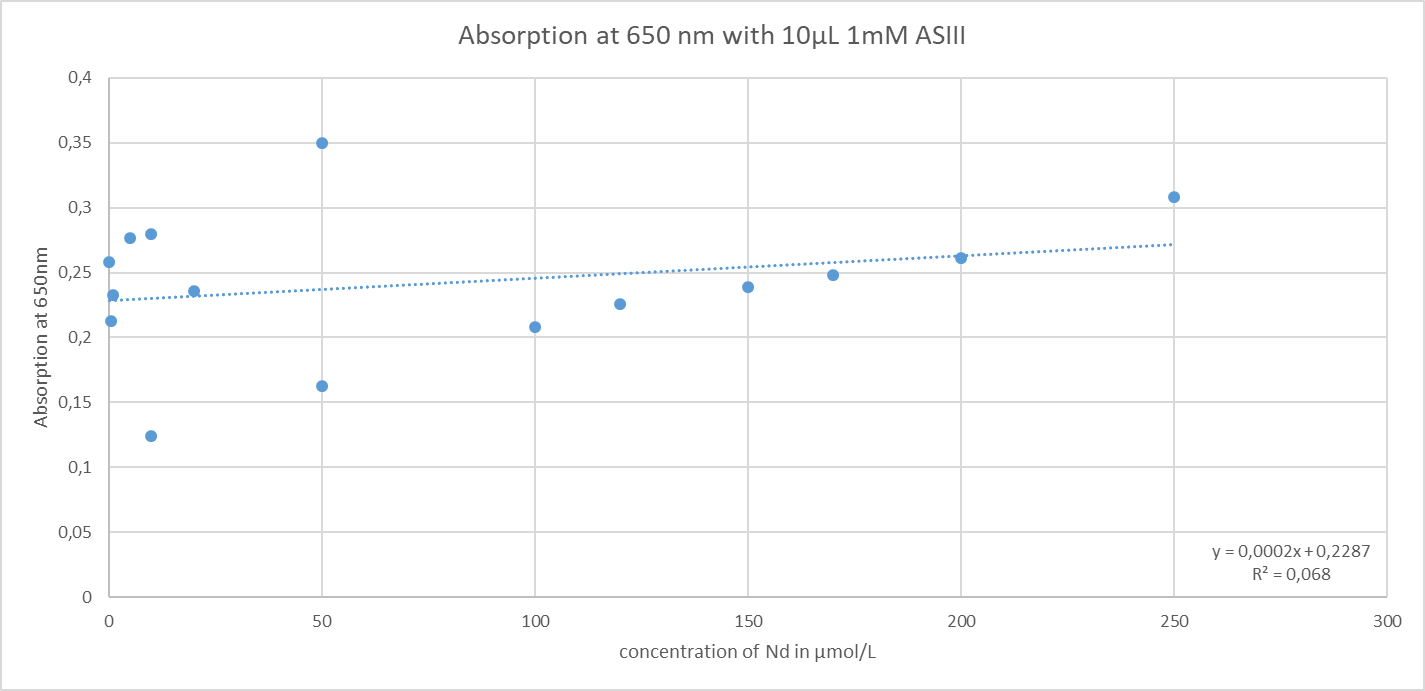
\includegraphics[width=1\textwidth]{./media/images/absorption10}
    \caption{Calibration line of absorption at 650nm with 10µL of 1mM arsenazo-III added.}
    \label{fig:absorption10}
\end{figure}

\begin{figure}[H]
    \centering
    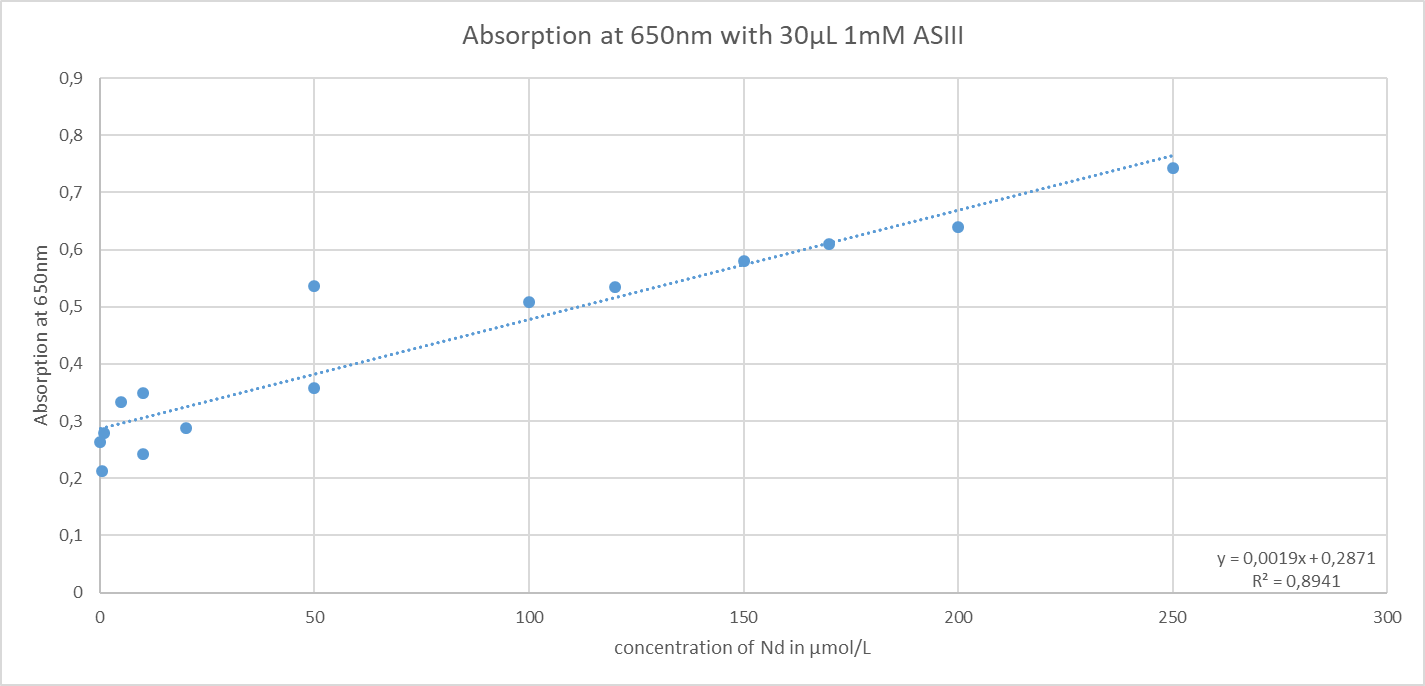
\includegraphics[width=1\textwidth]{media/images/absorption30}
    \caption{Calibration line of absorption at 650nm with 30µL of 1mM arsenazo-III added.}
    \label{fig:absorption30}
\end{figure}

In figure~\ref{fig:absorption10} it is clearly visible, that the values for the absorption fluctuate heavily.
The resulting calibration line should not be used for calculating the concentration.
Therefore, we used the graph in figure~\ref{fig:absorption30} to calculate the remaining concentration of \ce{Nd} in the nutrient solution.

\begin{table}[H]
    \centering
    \begin{tabularx}{\textwidth}{X X X X}
        \hline
        \textbf{Initial \ce{Nd} concentration} & \textbf{\ce{Nd} concentration after one week of bacteria growth} & \textbf{Absolute Change} & \textbf{Percentage change} \\ \hline
        0µmol/L & -39µmol/L & -39µmol/L & -\%\\
        200µmol/L & 49,68µmol/L & -150,32µmol/L & -75,16\% \\
        1mmol/L & 279,42µmol/L & -720,58µmol/L & -72,58\% \\
        \hline
    \end{tabularx}
    \caption{Initial and remaining concentration of \ce{Nd} in the nutrient solution.}
    \label{tab:nd_remaining}
\end{table}

In table~\ref{tab:nd_remaining}, \emph{M. extorquens} demonstrates its efficiency.
In just one week of growth, the bacteria were able to accumulate more than 70\% of neodymium in a solution.
It was irrelevant, how concentrated the neodymium was.

These results are very promising.
We did not only confirm that \emph{M. extorquens} is able to accumulate \ce{Nd} but without additional changes, it is naturally able to bind more than 70\% of the given neodymium.
